% begin module exponential-function-graphs
\begin{frame}
\begin{center}
Graphs of various exponential functions.

\psset{xunit=2cm, yunit=2cm}
\begin{pspicture}(-2.2, -0.3)(2.2,3.6) 
\psframe*[linecolor=white](-5,-5)(5,5) 
\psaxes[labels=none]{<->}(0,0)(-2.1,-0.2)(2.1,3.5)
\uncover<1->{
\rput[r](1.8, 2.3){$y=2^x$}
%Function formula: 2^{x} 
\psplot[linecolor=red, plotpoints=1000]{-2}{1.584962501}{2 x exp }
}
\uncover<2->{
\rput[l](1.2, 3.1){$y=4^x$}
%Function formula: 4^{x} 
\psplot[linecolor=black, plotpoints=1000]{-2}{0.79248125}{4 x exp }
}
\uncover<3->{
\rput[b](0.4, 3.05){$y=10^x$}
%Function formula: 4^{x} 
\psplot[linecolor=blue, plotpoints=1000]{-2}{0.477121255}{10 x exp }
}
\uncover<4->{
\rput[l](1.15, 1.5){$y=1.5^x$}
%Function formula: 4^{x} 
\psplot[linecolor=green, plotpoints=1000]{-2}{2}{1.5 x exp }
}
\uncover<5->{
\rput[l](-1.9, 2){$y=0.5^x$}
%Function formula: 4^{x} 
\psplot[linecolor=purple, plotpoints=1000]{-1.584962501}{2}{0.5 x exp }
}
\uncover<6->{
\rput[l](-1.2, 3.1){$y=0.25^x$}
%Function formula: 4^{x} 
\psplot[linecolor=brown, plotpoints=1000]{-0.79248125}{2}{0.25 x exp }
}
\end{pspicture}
\pause\pause\pause\pause\pause
%\ \only<handout:0| -1>{%
%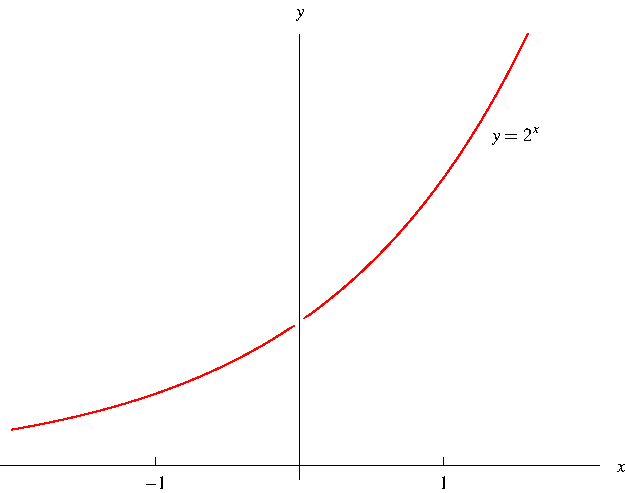
\includegraphics[height=6cm]{exponential-functions/pictures/07-02-manyexpa.pdf}%
%}%
%\only<handout:0| 2>{%
%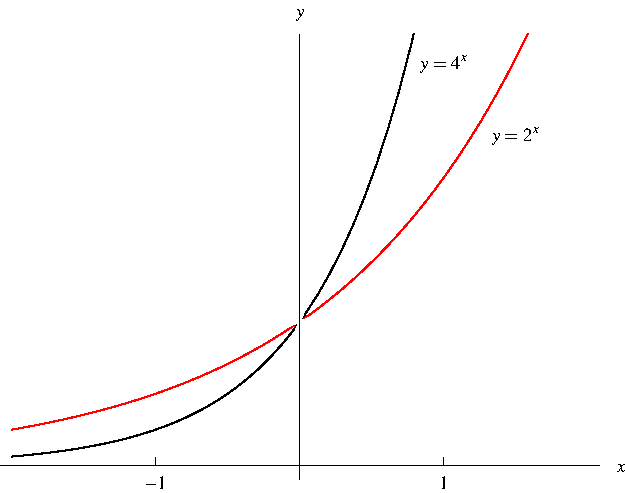
\includegraphics[height=6cm]{exponential-functions/pictures/07-02-manyexpb.pdf}%
%}%
%\only<handout:0| 3>{%
%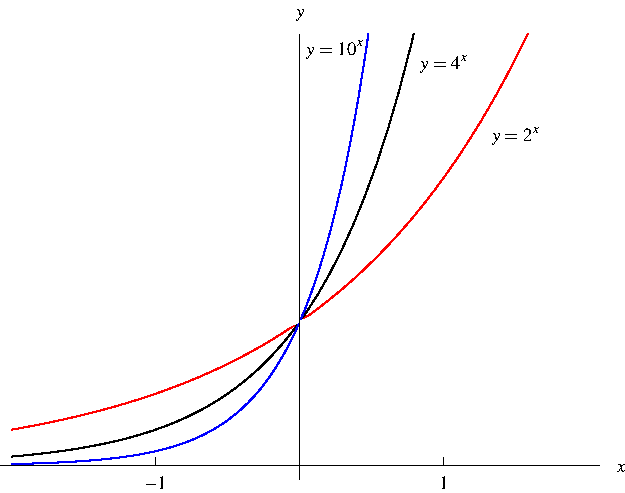
\includegraphics[height=6cm]{exponential-functions/pictures/07-02-manyexpc.pdf}%
%}%
%\only<handout:0| 4>{%
%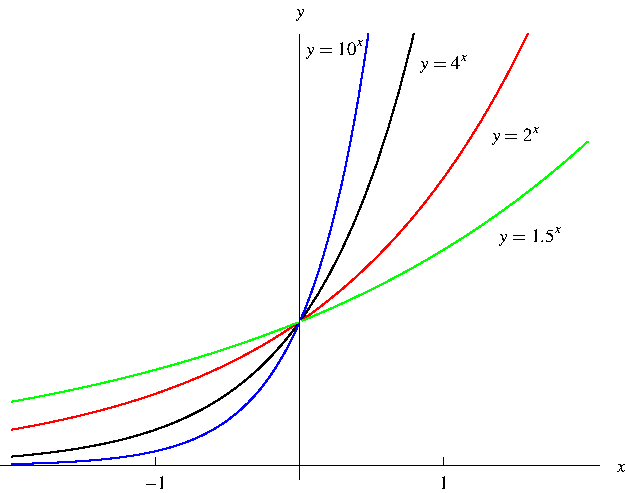
\includegraphics[height=6cm]{exponential-functions/pictures/07-02-manyexpd.pdf}%
%}%
%\only<handout:0| 5>{%
%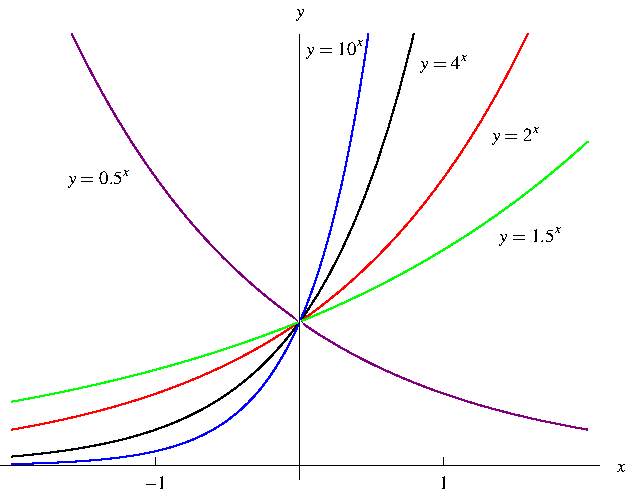
\includegraphics[height=6cm]{exponential-functions/pictures/07-02-manyexpe.pdf}%
%}%
%\only<6->{%
%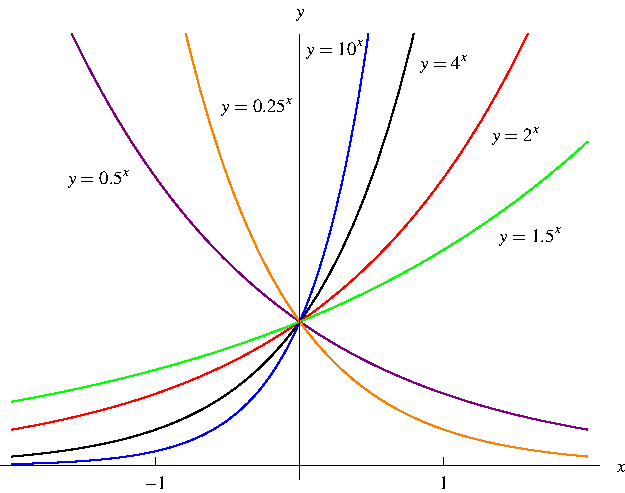
\includegraphics[height=6cm]{exponential-functions/pictures/07-02-manyexpf.pdf}%
%}%

\end{center}
\end{frame}
% end module exponential-function-graphs
